\documentclass[UTF8]{ctexart}
\usepackage{color}  
\usepackage{amsmath, bm}
\usepackage{graphicx}
\usepackage[colorlinks,linkcolor=red]{hyperref}

    \title{Get To The Point: Summarization with Pointer-Generator Networks}
    %\author{David}
    \date{\today}
    \begin{document}
    \maketitle
    \section{Abstract}
    \begin{itemize}
    \item  Neural sequence-to-sequence models have provided a viable new approach for ab-
    stractive text summarization (meaning they are not restricted to simply selecting
    and rearranging passages from the original text). \textcolor{red}{However, these models have two
    shortcomings: they are liable to reproduce factual details inaccurately, and they tend
    to repeat themselves.  }
    \item \textcolor{red}{In this work we propose a novel architecture that augments the
    standard sequence-to-sequence attentional model in two orthogonal ways. }
    \item \textcolor{red}{First,we use a hybrid pointer-generator network that can copy words from the source text
    via pointing, which aids accurate reproduction of information, while retaining the
    ability to produce novel words through the generator.} 
    \item \textcolor{red}{Second, we use coverage to keep track of what has been summarized,
    which discourages repetition.}
    \item We apply our model to the CNN \/ Daily Mail summarization task, outperforming the current
    abstractive state-of-the-art by at least 2 ROUGE points.
    \end{itemize}

    \section{Introduction}
    \begin{itemize}
    \item Summarization is the task of condensing a piece of text to a shorter version that contains the main in-
    formation from the original. There are two broad approaches to summarization: extractive and ab-
    stractive. Extractive methods assemble summaries exclusively from passages (usually whole sentences) taken directly from the source text, while
    abstractive methods may generate novel words and phrases not featured in the source text  as
    a human-written abstract usually does. 

    \item The extractive approach is easier, because copying large chunks of text from the source document ensures
    baseline levels of grammaticality and accuracy.On the other hand, sophisticated abilities that are
    crucial to high-quality summarization, such as paraphrasing, generalization, or the incorporation
    of real-world knowledge, are possible only in an abstractive framework (see Figure 5).
    
    \item Due to the difficulty of abstractive summarization, the great majority of past work has been ex-
    tractive (Kupiec et al., 1995; Paice, 1990; Saggion and Poibeau, 2013). However, the recent success of sequence-to-sequence models (Sutskever et al., 2014), in which recurrent neural networks
    (RNNs) both read and freely generate text, has made abstractive summarization viable (Chopra
    et al., 2016; Nallapati et al., 2016; Rush et al.,2015; Zeng et al., 2016). Though these systems
    are promising,\textcolor{red}{ they exhibit undesirable behavior such as inaccurately reproducing factual details,
    an inability to deal with out-of-vocabulary (OOV) words, and repeating themselves (see Figure 1)}

\begin{figure}[htbp]
  \centering
  \vspace{-0.35cm} 
  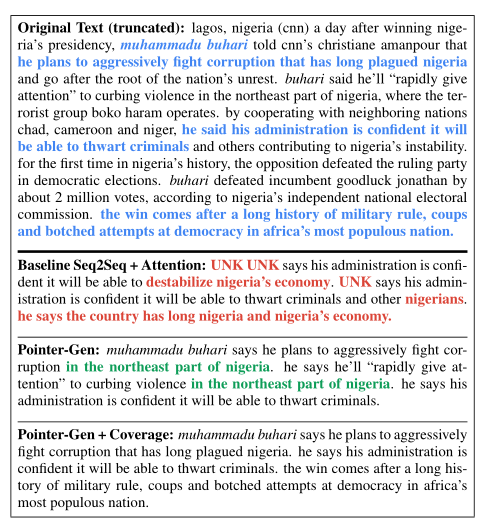
\includegraphics[width=11cm,height=13cm]{pictures/three.jpg}
  \caption{Comparison of output of 3 abstractive summarization models on a news article. The
  baseline model makes factual errors, a nonsensical sentence and struggles with OOV words
  muhammadu buhari. The pointer-generator model is accurate but repeats itself. Coverage eliminates
  repetition. The final summary is composed from several fragments.}
\end{figure}

    \item In this paper we present an architecture that
    addresses these three issues in the context of
    multi-sentence summaries. While most recent ab-
    stractive work has focused on headline genera-
    tion tasks (reducing one or two sentences to a
    single headline), we believe that longer-text sum-
    marization is both more challenging (requiring
    higher levels of abstraction while avoiding repe-
    tition) and ultimately more useful. Therefore we
    apply our model to the recently-introduced CNN/
    Daily Mail dataset (Hermann et al., 2015; Nallap-
    ati et al., 2016), which contains news articles (39
    sentences on average) paired with multi-sentence
    summaries, and show that we outperform the state-
    of-the-art abstractive system by at least 2 ROUGE
    points.

    \item  Our hybrid pointer-generator network facilitates copying words from the source text via point-
    ing (Vinyals et al., 2015), which improves accuracy and handling of OOV words, while retaining
    the ability to generate new words. The network,which can be viewed as a balance between extrac-
    tive and abstractive approaches, is similar to Gu et al.s (2016) CopyNet and Miao and Blunsoms
    (2016) Forced-Attention Sentence Compression,that were applied to short-text summarization. We
    propose a novel variant of the coverage vector (Tu et al., 2016) from Neural Machine Translation,
    which we use to track and control coverage of the source document. We show that coverage is re-
    markably effective for eliminating repetition.
    \end{itemize}

    \section{Our Models}
    In this section we describe (1) our baseline sequence-to-sequence model, (2) our pointer-
    generator model, and (3) our coverage mechanism that can be added to either of the first two models.
    The code for our models is available online.1

    \subsection{Sequence-to-sequence attentional model}
    Our baseline model is similar to that of Nallapati
et al. (2016), and is depicted in Figure 2. The to-
kens of the article wi are fed one-by-one into the
encoder (a single-layer bidirectional LSTM), pro-
ducing a sequence of encoder hidden states $h_i$. On
each step $t$, the decoder (a single-layer unidirec-
tional LSTM) receives the word embedding of the
previous word (while training, this is the previous
word of the reference summary; at test time it is
the previous word emitted by the decoder), and
has decoder state $s_t$. The attention distribution at
is calculated as in Bahdanau et al. (2015):

$    {e_i}^t=v_Ttanh(W_h h_i +W_s s_t + b_attn)  $

$     a_t=softmax(e^t)   $

where $v$, $W_h$, $W_s$ and $b_attn$ are learnable parame-
ters. The attention distribution can be viewed as a probability distribution over the source words,
that tells the decoder where to look to produce the
next word. Next, the attention distribution is used
to produce a weighted sum of the encoder hidden
states, known as the context vector ${h_t}^*$ :

$    {h_t}^*=\sum_{i}{a_i}^t h_i$

The context vector, which can be seen as a fixed-size representation of what has been read from the
source for this step, is concatenated with the decoder state $s_t$ and fed through two linear layers to
produce the vocabulary distribution $P_vocab$:

$   P_vocab =softmax(V'(V[s_t,{h_t}^*]+b)+b')  $

where $V , V', b$ and $b'$ are learnable parameters.
$P_vocab$ is a probability distribution over all words
in the vocabulary, and provides us with our final
distribution from which to predict words $w$:


$ P(w)=P_vocab(w)  $

During training, the loss for timestep $t$ is the negative log likelihood of the target word ${w_t}^*$ for that
timestep:

$ loss_t=-logP({w_t}^*) $

and the overall loss for the whole sequence is:

$ loss=\frac{1}{T}\sum_{t=0}^{T}loss_t  $

   \subsection{Pointer-generator network}

   Our pointer-generator network is a hybrid between
our baseline and a pointer network (Vinyals et al.,
2015), as it allows both copying words via pointing, and generating words from a fixed vocabulary.
In the pointer-generator model (depicted in Figure3) the attention distribution $a_t$ and context vector
${h_t}^*$ are calculated as in section 2.1. In addition, the
generation probability $p_gen \in [0,1]$ for timestep t is
calculated from the context vector ${h_t}^*$ , the decoder
state $s_t$ and the decoder input $x_t$:

$ p_gen = \sigma ({w_h*}^T {h_t}^* +  {w_s}^T s_t  +  {w_x}^T x_t +b_ptr) $


where vectors $w_h*, w_s, w_x$ and scalar $b_ptr$ are learn-
able parameters and $\sigma$ is the sigmoid function.
Next, $p_gen$ is used as a soft switch to choose be-
tween generating a word from the vocabulary by
sampling from $P_vocab$, or copying a word from the
input sequence by sampling from the attention dis-
tribution $a_t$. For each document let the extended
vocabulary denote the union of the vocabulary,
and all words appearing in the source document.
We obtain the following probability distribution
over the extended vocabulary:

$    P(w)=p_gen P_vocab(w) +(1-p_gen)\sum_{i:w_i=w}{a_i}^t $


Note that if w is an out-of-vocabulary (OOV)
word, then $P_vocab(w)$ is zero; similarly if w does
not appear in the source document, then $\sum_{i:w_i=w}{a_i}^t$
is zero. The ability to produce OOV words is
one of the primary advantages of pointer-generator
models; by contrast models such as our baseline
are restricted to their pre-set vocabulary.
The loss function is as described in equations
(6) and (7), but with respect to our modified prob-
ability distribution P(w) given in equation (9).


   \subsection{Coverage mechanism}

   Repetition is a common problem for sequence-
to-sequence models (Tu et al., 2016; Mi et al.,
2016; Sankaran et al., 2016; Suzuki and Nagata,
2016), and is especially pronounced when gener-
ating multi-sentence text (see Figure 1). We adapt
the coverage model of Tu et al. (2016) to solve the
problem. In our coverage model, we maintain a
coverage vector $c_t$, which is the sum of attention
distributions over all previous decoder timesteps:

$             c_t=\sum_{t'=0}^{t-1} a_t'    $

Intuitively, $c_t$ is a (unnormalized) distribution over
the source document words that represents the degree of coverage that those words have received
from the attention mechanism so far. Note that $c^0$
is a zero vector, because on the first timestep, none
of the source document has been covered.

The coverage vector is used as extra input to the
attention mechanism, changing equation (1) to:

$  {e_i}_t=v^Ttanh(W_h h_i+ W_s s_t +w_c {c_i}^t +b_attn )$

where $w_c$ is a learnable parameter vector of same
length as v. This ensures that the attention mecha-
nism’s current decision (choosing where to attend
next) is informed by a reminder of its previous
decisions (summarized in $c_t$). This should make
it easier for the attention mechanism to avoid re-
peatedly attending to the same locations, and thus
avoid generating repetitive text.

We find it necessary (see section 5) to addition-
ally define a coverage loss to penalize repeatedly
attending to the same locations:


$ covloss_t=\sum_{t}min({a_i}^t,{a_i}^t)                                         $

Note that the coverage loss is bounded; in particu-
lar $covloss_t ≤ \sum_{i} {a_i}^t=1$. Equation (12) differs from
the coverage loss used in Machine Translation. In
MT, we assume that there should be a roughly one-
to-one translation ratio; accordingly the final cov-
erage vector is penalized if it is more or less than 1.
Our loss function is more flexible: because sum-
marization should not require uniform coverage,
we only penalize the overlap between each atten-
tion distribution and the coverage so far – prevent-
ing repeated attention. Finally, the coverage loss,
reweighted by some hyperparameter $\lambda$, is added to
the primary loss function to yield a new composite
loss function:

$  loss_t=-logP({w_t}^*)+\lambda \sum_{i}min({a_i}^t,{c_i}^t)                             $



   \section{Related Work}

   Neural abstractive summarization. Rush et al.
(2015) were the first to apply modern neural net-
works to abstractive text summarization, achiev-
ing state-of-the-art performance on DUC-2004
and Gigaword, two sentence-level summarization
datasets. Their approach, which is centered on the
attention mechanism, has been augmented with re-
current decoders (Chopra et al., 2016), Abstract
Meaning Representations (Takase et al., 2016), hi-
erarchical networks (Nallapati et al., 2016), vari-
ational autoencoders (Miao and Blunsom, 2016),
and direct optimization of the performance metric
(Ranzato et al., 2016), further improving perfor-
mance on those datasets.


However, large-scale datasets for summariza-
tion of longer text are rare. Nallapati et al. (2016)
adapted the DeepMind question-answering dataset
(Hermann et al., 2015) for summarization, result-
ing in the CNN/Daily Mail dataset, and provided
the first abstractive baselines. The same authors
then published a neural extractive approach (Nal-
lapati et al., 2017), which uses hierarchical RNNs
to select sentences, and found that it significantly
outperformed their abstractive result with respect
to the ROUGE metric. To our knowledge, these
are the only two published results on the full data-
set.

Prior to modern neural methods, abstractive
summarization received less attention than extrac-
tive summarization, but Jing (2000) explored cut-
ting unimportant parts of sentences to create sum-
maries, and Cheung and Penn (2014) explore sen-
tence fusion using dependency trees.

Pointer-generator networks. The pointer net-
work (Vinyals et al., 2015) is a sequence-to-
sequence model that uses the soft attention dis-
tribution of Bahdanau et al. (2015) to produce
an output sequence consisting of elements from

the input sequence. The pointer network has been
used to create hybrid approaches for NMT (Gul-
cehre et al., 2016), language modeling (Merity
et al., 2016), and summarization (Gu et al., 2016;
Gulcehre et al., 2016; Miao and Blunsom, 2016;
Nallapati et al., 2016; Zeng et al., 2016).


Our approach is close to the Forced-Attention
Sentence Compression model of Miao and Blun-
som (2016) and the CopyNet model of Gu et al.
(2016), with some small differences: (i) We cal-
culate an explicit switch probability pgen, whereas
Gu et al. induce competition through a shared soft-
max function. (ii) We recycle the attention distri-
bution to serve as the copy distribution, but Gu et
al. use two separate distributions. (iii) When a
word appears multiple times in the source text, we
sum probability mass from all corresponding parts
of the attention distribution, whereas Miao and
Blunsom do not. Our reasoning is that (i) calcu-
lating an explicit pgen usefully enables us to raise
or lower the probability of all generated words or
all copy words at once, rather than individually,
(ii) the two distributions serve such similar pur-
poses that we find our simpler approach suffices,
and (iii) we observe that the pointer mechanism
often copies a word while attending to multiple oc-
currences of it in the source text.


Our approach is considerably different from
that of Gulcehre et al. (2016) and Nallapati et al.
(2016). Those works train their pointer compo-
nents to activate only for out-of-vocabulary words
or named entities (whereas we allow our model to
freely learn when to use the pointer), and they do
not mix the probabilities from the copy distribu-
tion and the vocabulary distribution. We believe
the mixture approach described here is better for
abstractive summarization – in section 6 we show
that the copy mechanism is vital for accurately
reproducing rare but in-vocabulary words, and in
section 7.2 we observe that the mixture model en-
ables the language model and copy mechanism to
work together to perform abstractive copying.


Coverage. Originating from Statistical Ma-
chine Translation (Koehn, 2009), coverage was
adapted for NMT by Tu et al. (2016) and Mi et al.
(2016), who both use a GRU to update the cov-
erage vector each step. We find that a simpler
approach – summing the attention distributions to
obtain the coverage vector – suffices. In this re-
spect our approach is similar to Xu et al. (2015),
who apply a coverage-like method to image cap-tioning, and Chen et al. (2016), who also incorpo-
rate a coverage mechanism (which they call ‘dis-
traction’) as described in equation (11) into neural
summarization of longer text.
Temporal attention is a related technique that
has been applied to NMT (Sankaran et al., 2016)
and summarization (Nallapati et al., 2016). In
this approach, each attention distribution is di-
vided by the sum of the previous, which effec-
tively dampens repeated attention. We tried this
method but found it too destructive, distorting the
signal from the attention mechanism and reducing
performance. We hypothesize that an early inter-
vention method such as coverage is preferable to
a post hoc method such as temporal attention – it
is better to inform the attention mechanism to help
it make better decisions, than to override its de-
cisions altogether. This theory is supported by the
large boost that coverage gives our ROUGE scores
(see Table 1), compared to the smaller boost given
by temporal attention for the same task (Nallapati
et al., 2016).




   \section{Dataset}

   We use the CNN/Daily Mail dataset (Hermann
et al., 2015; Nallapati et al., 2016), which con-
tains online news articles (781 tokens on average)
paired with multi-sentence summaries (3.75 sen-
tences or 56 tokens on average). We used scripts
supplied by Nallapati et al. (2016) to obtain the
same version of the the data, which has 287,226
training pairs, 13,368 validation pairs and 11,490
test pairs. Both the dataset  s published results
(Nallapati et al., 2016, 2017) use the anonymized
version of the data, which has been pre-processed
to replace each named entity, e.g., The United Na-
tions, with its own unique identifier for the exam-
ple pair, e.g., @entity5. By contrast, we operate
directly on the original text (or non-anonymized
version of the data),2 which we believe is the fa-
vorable problem to solve because it requires no
pre-processing.


    \section{Experiments}

    \section{Results}


    \section{Discussion}

    \subsubsection{Comparison with extractive systems}
    It is clear from Table 1 that extractive systems tend
to achieve higher ROUGE scores than abstractive,
and that the extractive lead-3 baseline is extremely
strong (even the best extractive system beats it by
only a small margin). We offer two possible ex-
planations for these observations.

Firstly, news articles tend to be structured with
the most important information at the start; this
partially explains the strength of the lead-3 base-
line. Indeed, we found that using only the first 400
tokens (about 20 sentences) of the article yielded
significantly higher ROUGE scores than using the
first 800 tokens.

Secondly, the nature of the task and the ROUGE
metric make extractive approaches and the lead-
3 baseline difficult to beat. The choice of con-
tent for the reference summaries is quite subjective
– sometimes the sentences form a self-contained
summary; other times they simply showcase a few
interesting details from the article. Given that the
articles contain 39 sentences on average, there are
many equally valid ways to choose 3 or 4 high-
lights in this style. Abstraction introduces even
more options (choice of phrasing), further decreasing the likelihood of matching the reference sum-
mary. For example, smugglers profit from des-
perate migrants is a valid alternative abstractive
summary for the first example in Figure 5, but
it scores 0 ROUGE with respect to the reference
summary. This inflexibility of ROUGE is exac-
erbated by only having one reference summary,
which has been shown to lower ROUGE’s relia-
bility compared to multiple reference summaries
(Lin, 2004a).

Due to the subjectivity of the task and thus
the diversity of valid summaries, it seems that
ROUGE rewards safe strategies such as select-
ing the first-appearing content, or preserving orig-
inal phrasing. While the reference summaries do
sometimes deviate from these techniques, those
deviations are unpredictable enough that the safer
strategy obtains higher ROUGE scores on average.
This may explain why extractive systems tend to
obtain higher ROUGE scores than abstractive, and
even extractive systems do not significantly ex-
ceed the lead-3 baseline.


To explore this issue further, we evaluated our
systems with the METEOR metric, which rewards
not only exact word matches, but also matching
stems, synonyms and paraphrases (from a pre-
defined list). We observe that all our models re-
ceive over 1 METEOR point boost by the inclu-
sion of stem, synonym and paraphrase matching,
indicating that they may be performing some ab-
straction. However, we again observe that the
lead-3 baseline is not surpassed by our models.
It may be that news article style makes the lead-
3 baseline very strong with respect to any metric.
We believe that investigating this issue further is
an important direction for future work.
   \subsection{How abstractive is our model?}
   We have shown that our pointer mechanism makes
our abstractive system more reliable, copying fac-
tual details correctly more often. But does the ease
of copying make our system any less abstractive?

Figure 6 shows that our final model’s sum-
maries contain a much lower rate of novel n-grams
(i.e., those that don’t appear in the article) than the
reference summaries, indicating a lower degree of
abstraction. Note that the baseline model produces
novel n-grams more frequently – however, this
statistic includes all the incorrectly copied words,
UNK tokens and fabrications alongside the good
instances of abstraction.

Figure 6: Although our best model is abstractive,
it does not produce novel n-grams (i.e., n-grams
that don’t appear in the source text) as often as
the reference summaries. The baseline model
produces more novel n-grams, but many of these
are erroneous (see section 7.2).

In particular, Figure 6 shows that our final
model copies whole article sentences 35\% of the
time; by comparison the reference summaries do
so only 1.3\% of the time. This is a main area for
improvement, as we would like our model to move
beyond simple sentence extraction. However, we
observe that the other 65\% encompasses a range of
abstractive techniques. Article sentences are trun-
cated to form grammatically-correct shorter ver-
sions, and new sentences are composed by stitch-
ing together fragments. Unnecessary interjections,
clauses and parenthesized phrases are sometimes
omitted from copied passages. Some of these abil-
ities are demonstrated in Figure 1, and the supple-
mentary material contains more examples.

Figure 7 shows two examples of more impres-
sive abstraction – both with similar structure. The
dataset contains many sports stories whose sum-
maries follow the X beat Y hscorei on hdayi template, which may explain why our model is most
confidently abstractive on these examples. In gen-
eral however, our model does not routinely pro-
duce summaries like those in Figure 7, and is not
close to producing summaries like in Figure 5.


The value of the generation probability pgen
also gives a measure of the abstractiveness of our
model. During training, pgen starts with a value
of about 0.30 then increases, converging to about
0.53 by the end of training. This indicates that
the model first learns to mostly copy, then learns
to generate about half the time. However at test
time, pgen is heavily skewed towards copying, with
a mean value of 0.17. The disparity is likely
due to the fact that during training, the model re-
ceives word-by-word supervision in the form of
the reference summary, but at test time it does
not. Nonetheless, the generator module is use-
ful even when the model is copying. We find
that pgen is highest at times of uncertainty such
as the beginning of sentences, the join between
stitched-together fragments, and when producing
periods that truncate a copied sentence. Our mix-
ture model allows the network to copy while si-
multaneously consulting the language model – en-
abling operations like stitching and truncation to
be performed with grammaticality. In any case,
encouraging the pointer-generator model to write
more abstractively, while retaining the accuracy
advantages of the pointer module, is an exciting
direction for future work.


    \section{Conclusion}

    In this work we presented a hybrid pointer-
generator architecture with coverage, and showed
that it reduces inaccuracies and repetition. We ap-
plied our model to a new and challenging long-
text dataset, and significantly outperformed the
abstractive state-of-the-art result. Our model ex-
hibits many abstractive abilities, but attaining
higher levels of abstraction remains an open re-
search question.



    \section{Personal understanding}

    \subsection{Paper structure}



    \subsection{The problem to solve}

    Problem 1: The summaries sometimes reproduce factual details inaccurately (e.g. Germany beat Argentina 3-2). This is especially common for rare or out-of-vocabulary words such as 2-0.

    Problem 2: The summaries sometimes repeat themselves (e.g. Germany beat Germany beat Germany beat…)

    Explanation for Problem 1: The sequence-to-sequence-with-attention model makes it too difficult to copy a word w from the source text. The network must somehow recover the original word after the information has passed through several layers of computation (including mapping w to its word embedding).
In particular, if w is a rare word that appeared infrequently during training and therefore has a poor word embedding (i.e. it is clustered with completely unrelated words), then w is, from the perspective of the network, indistinguishable from many other words, thus impossible to reproduce.
Even if w has a good word embedding, the network may still have difficulty reproducing the word. For example, RNN summarization systems often replace a name with another name (e.g. Anna → Emily) or a city with another city (e.g. Delhi → Mumbai). This is because the word embeddings for e.g. female names or Indian cities tend to cluster together, which may cause confusion when attempting to reconstruct the original word.
In short, this seems like an unnecessarily difficult way to perform a simple operation – copying – that is a fundamental operation in summarization.

Explanation for Problem 2: Repetition may be caused by the decoder’s over-reliance on the decoder input (i.e. previous summary word), rather than storing longer-term information in the decoder state. This can be seen by the fact that a single repeated word commonly triggers an endless repetitive cycle. For example, a single substitution error Germany beat Germany leads to the catastrophic Germany beat Germany beat Germany beat…, and not the less-wrong Germany beat Germany 2-0.



    \subsection{The innovation work}

    \begin{figure}[htbp]
        \centering
        \vspace{-0.35cm} 
        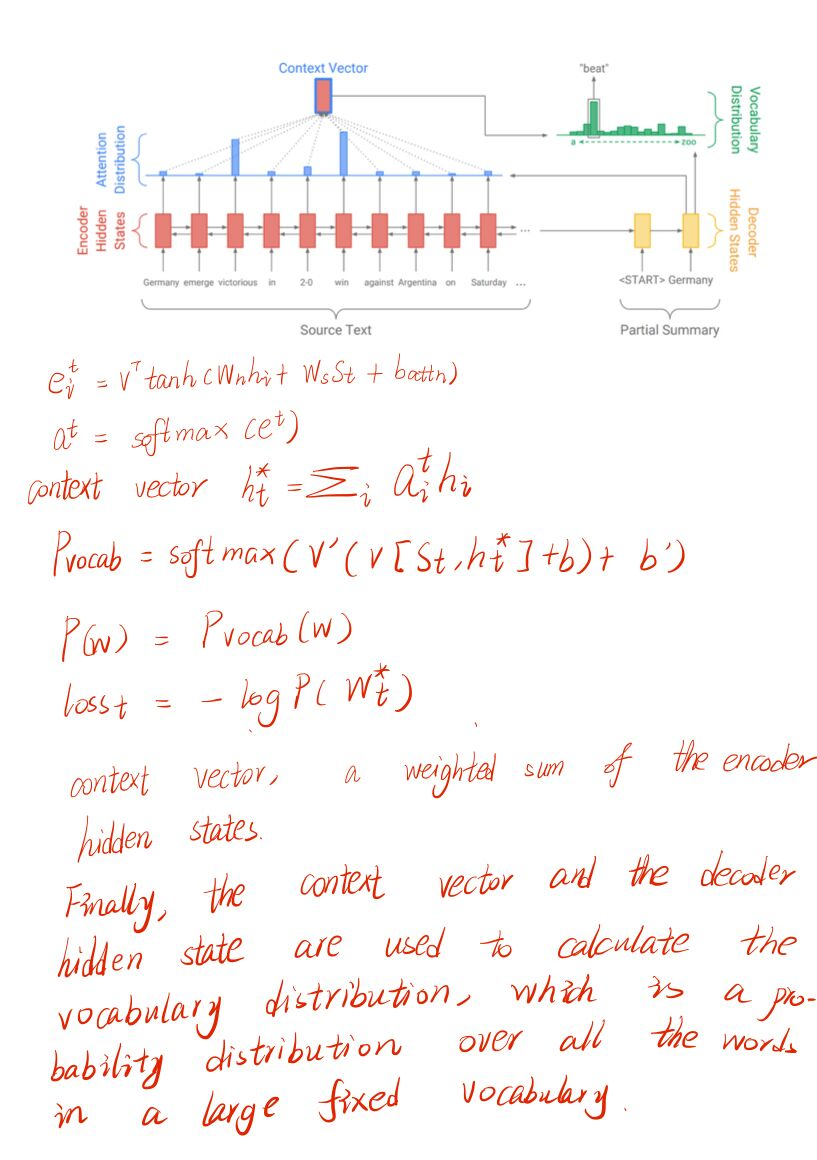
\includegraphics[width=14cm,height=18cm]{pictures/11.jpg}
        \caption{Baseline sequence-to-sequence model with attention. The model may attend to relevant words
        in the source text to generate novel words, e.g., to produce the novel word beat in the abstractive summary
        Germany beat Argentina 2-0 the model may attend to the words victorious and win in the source text.}
    \end{figure}


    \begin{figure}[htbp]
        \centering
        \vspace{-0.35cm} 
        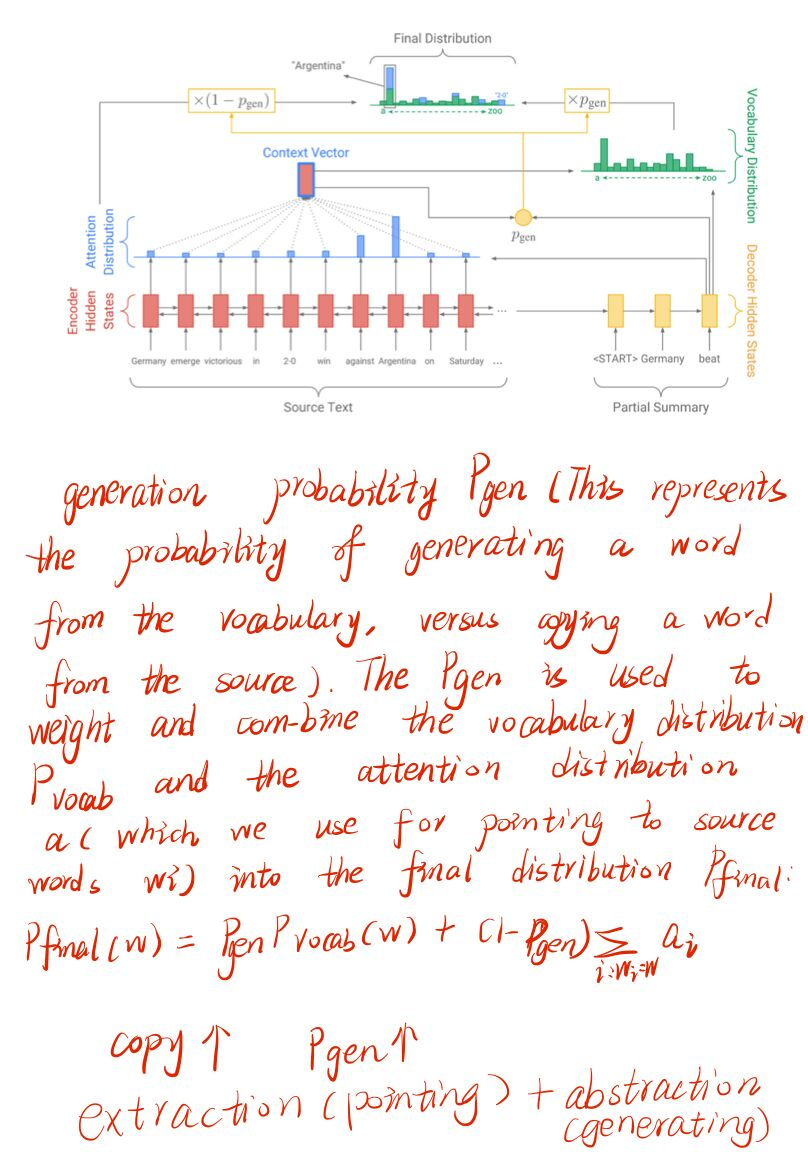
\includegraphics[width=14cm,height=18cm]{pictures/22.jpg}
        \caption{Pointer-generator model. For each decoder timestep a generation probability pgen ∈ [0,1] is
        calculated, which weights the probability of generating words from the vocabulary, versus copying words
        from the source text. The vocabulary distribution and the attention distribution are weighted and summed
        to obtain the final distribution, from which we make our prediction. Note that out-of-vocabulary article
        words such as 2-0 are included in the final distribution. Best viewed in color.}
    \end{figure}

    \begin{figure}[htbp]
        \centering
        \vspace{-0.35cm} 
        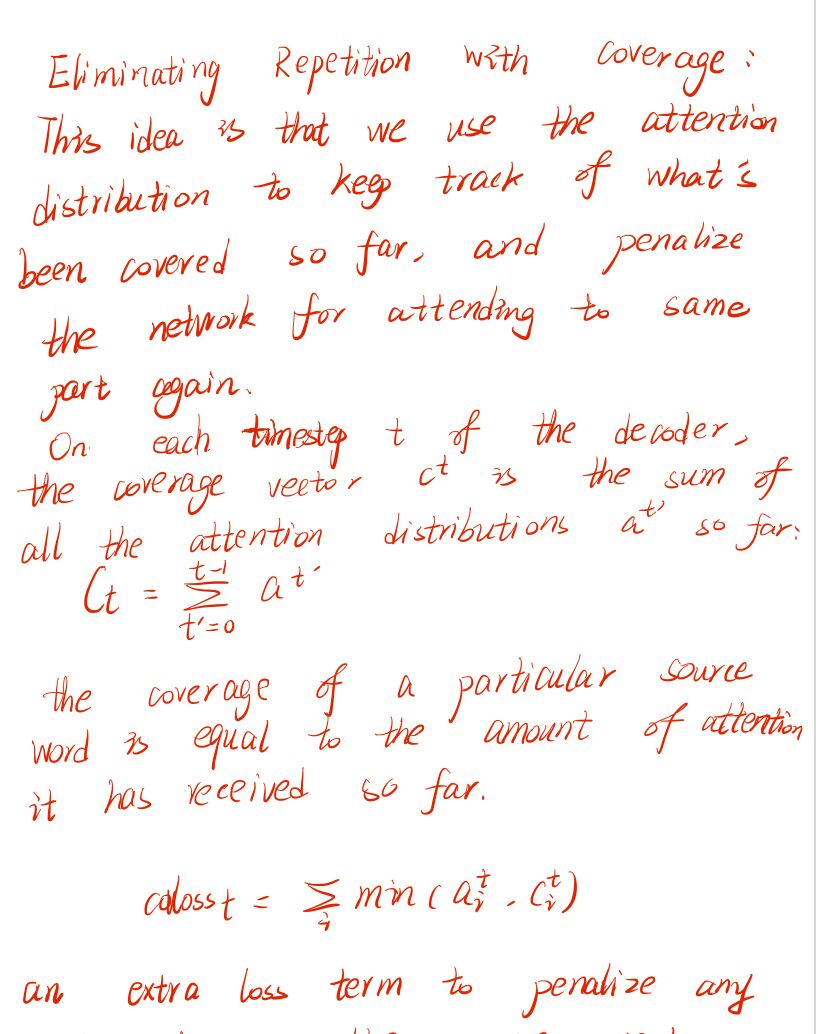
\includegraphics[width=14cm,height=18cm]{pictures/33.jpg}
        \caption{Coverage mechanism}
    \end{figure}



  
    \subsection{The code analysis}

    \url{http://www.abigailsee.com/2017/04/16/taming-rnns-for-better-summarization.html}

    \url{https://github.com/abisee/pointer-generator}



    \end{document}

